\section{eo\-Populator$<$ EOT $>$ Class Template Reference}
\label{classeo_populator}\index{eoPopulator@{eoPopulator}}
eo\-Populator is a helper class for general operators {\bf eo\-Gen\-Op}{\rm (p.\,\pageref{classeo_gen_op})} It is an {\bf eo\-Pop}{\rm (p.\,\pageref{classeo_pop})} but also behaves like an eo\-Pop::iterator as far as operator$\ast$ and operator++ are concerned  


{\tt \#include $<$eo\-Populator.h$>$}

Inheritance diagram for eo\-Populator$<$ EOT $>$::\begin{figure}[H]
\begin{center}
\leavevmode
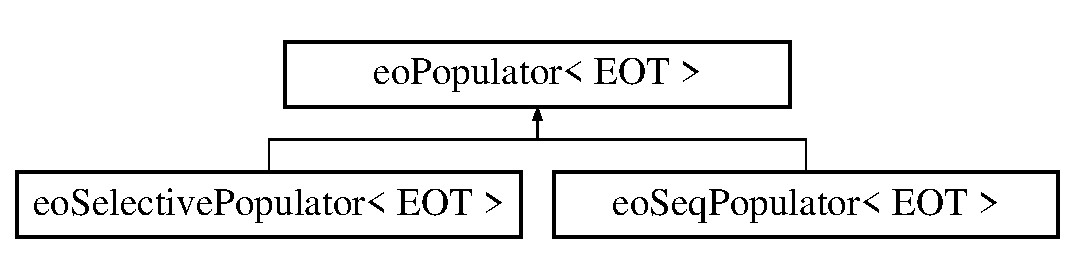
\includegraphics[height=2cm]{classeo_populator}
\end{center}
\end{figure}
\subsection*{Public Types}
\begin{CompactItemize}
\item 
typedef unsigned {\bf position\_\-type}\label{classeo_populator_w0}

\end{CompactItemize}
\subsection*{Public Member Functions}
\begin{CompactItemize}
\item 
{\bf eo\-Populator} (const {\bf eo\-Pop}$<$ {\bf EOT} $>$ \&\_\-src, {\bf eo\-Pop}$<$ {\bf EOT} $>$ \&\_\-dest)\label{classeo_populator_a0}

\item 
virtual {\bf $\sim$eo\-Populator} ()\label{classeo_populator_a1}

\begin{CompactList}\small\item\em Virtual Constructor. \item\end{CompactList}\item 
{\bf EOT} \& {\bf operator $\ast$} (void)
\begin{CompactList}\small\item\em a populator behaves like an iterator. \item\end{CompactList}\item 
{\bf eo\-Populator} \& {\bf operator++} ()\label{classeo_populator_a3}

\begin{CompactList}\small\item\em only prefix increment defined Does not add a new element when at the end, use operator$\ast$ for that If not on the end, increment the pointer to the next individual \item\end{CompactList}\item 
void {\bf insert} (const {\bf EOT} \&\_\-eo)\label{classeo_populator_a4}

\begin{CompactList}\small\item\em mandatory for operators that generate more offspring than parents if such a thing exists ? \item\end{CompactList}\item 
void {\bf reserve} (int how\_\-many)\label{classeo_populator_a5}

\begin{CompactList}\small\item\em just to make memory mangement more efficient \item\end{CompactList}\item 
const {\bf eo\-Pop}$<$ {\bf EOT} $>$ \& {\bf source} (void)
\begin{CompactList}\small\item\em can be useful for operators with embedded selectors e.g. \item\end{CompactList}\item 
{\bf eo\-Pop}$<$ {\bf EOT} $>$ \& {\bf offspring} (void)
\begin{CompactList}\small\item\em Get the offspring population. \item\end{CompactList}\item 
position\_\-type {\bf tellp} ()\label{classeo_populator_a8}

\begin{CompactList}\small\item\em this is a direct access container: tell position \item\end{CompactList}\item 
void {\bf seekp} (position\_\-type pos)\label{classeo_populator_a9}

\begin{CompactList}\small\item\em this is a direct access container: go to position \item\end{CompactList}\item 
bool {\bf exhausted} (void)\label{classeo_populator_a10}

\begin{CompactList}\small\item\em no more individuals \item\end{CompactList}\item 
virtual const {\bf EOT} \& {\bf select} ()=0\label{classeo_populator_a11}

\begin{CompactList}\small\item\em the pure virtual selection method - will be instanciated in {\bf eo\-Seq\-Populator}{\rm (p.\,\pageref{classeo_seq_populator})} and {\bf eo\-Selective\-Populator}{\rm (p.\,\pageref{classeo_selective_populator})} \item\end{CompactList}\end{CompactItemize}
\subsection*{Protected Attributes}
\begin{CompactItemize}
\item 
{\bf eo\-Pop}$<$ {\bf EOT} $>$ \& {\bf dest}\label{classeo_populator_p0}

\item 
{\bf eo\-Pop}$<$ {\bf EOT} $>$::iterator {\bf current}\label{classeo_populator_p1}

\item 
const {\bf eo\-Pop}$<$ {\bf EOT} $>$ \& {\bf src}\label{classeo_populator_p2}

\end{CompactItemize}
\subsection*{Private Member Functions}
\begin{CompactItemize}
\item 
void {\bf get\_\-next} ()\label{classeo_populator_d0}

\end{CompactItemize}


\subsection{Detailed Description}
\subsubsection*{template$<$class EOT$>$ class eo\-Populator$<$ EOT $>$}

eo\-Populator is a helper class for general operators {\bf eo\-Gen\-Op}{\rm (p.\,\pageref{classeo_gen_op})} It is an {\bf eo\-Pop}{\rm (p.\,\pageref{classeo_pop})} but also behaves like an eo\-Pop::iterator as far as operator$\ast$ and operator++ are concerned 

See {\bf eo\-Gen\-Op}{\rm (p.\,\pageref{classeo_gen_op})} and {\bf eo\-Op\-Container}{\rm (p.\,\pageref{classeo_op_container})} 



Definition at line 39 of file eo\-Populator.h.

\subsection{Member Function Documentation}
\index{eoPopulator@{eo\-Populator}!operator *@{operator $\ast$}}
\index{operator *@{operator $\ast$}!eoPopulator@{eo\-Populator}}
\subsubsection{\setlength{\rightskip}{0pt plus 5cm}template$<$class EOT$>$ {\bf EOT}\& {\bf eo\-Populator}$<$ {\bf EOT} $>$::operator $\ast$ (void)\hspace{0.3cm}{\tt  [inline]}}\label{classeo_populator_a2}


a populator behaves like an iterator. 

Hence the operator$\ast$ it returns the current individual -- eventually getting a new one through the operator++ if at the end 

Definition at line 58 of file eo\-Populator.h.\index{eoPopulator@{eo\-Populator}!source@{source}}
\index{source@{source}!eoPopulator@{eo\-Populator}}
\subsubsection{\setlength{\rightskip}{0pt plus 5cm}template$<$class EOT$>$ const {\bf eo\-Pop}$<${\bf EOT}$>$\& {\bf eo\-Populator}$<$ {\bf EOT} $>$::source (void)\hspace{0.3cm}{\tt  [inline]}}\label{classeo_populator_a6}


can be useful for operators with embedded selectors e.g. 

your brain and my beauty -type 

Definition at line 105 of file eo\-Populator.h.

Referenced by eo\-Sel\-Bin\-Gen\-Op$<$ EOT $>$::apply(), and eo\-Es\-Global\-Xover$<$ EOT $>$::apply().\index{eoPopulator@{eo\-Populator}!offspring@{offspring}}
\index{offspring@{offspring}!eoPopulator@{eo\-Populator}}
\subsubsection{\setlength{\rightskip}{0pt plus 5cm}template$<$class EOT$>$ {\bf eo\-Pop}$<${\bf EOT}$>$\& {\bf eo\-Populator}$<$ {\bf EOT} $>$::offspring (void)\hspace{0.3cm}{\tt  [inline]}}\label{classeo_populator_a7}


Get the offspring population. 

Can be useful when you want to do some online niching kind of thing 

Definition at line 110 of file eo\-Populator.h.

The documentation for this class was generated from the following file:\begin{CompactItemize}
\item 
eo\-Populator.h\end{CompactItemize}
